\documentclass[10pt, uplatex, dvipdfmx]{jsarticle}
\usepackage{../mypackage}

\graphicspath{{../pictures}}

\setcounter{section}{13}

\begin{document}


\section{数値積分}

積分 $\ds \int_{a}^{b} f(x) \ dx$ の値を知りたければ,$f$ の原始関数,つまり $F'=f$ となる関数 $F$ を見つけて
\[
  \int_{a}^{b} f(x) \ dx = F(b) - F(a)
\]
と計算することができる,とういのが微分積分学の基本定理の使い方だった.
しかしながら,例えば以下のような積分に対してはこの方法は通用しない.
\[
  \int_{0}^{1} e^{-x^2} \ dx, \quad \int_{0}^{1} \frac{\sin x}{x} \ dx, \quad \int_{2}^{3} \frac{dx}{\log x}
\]
また,微分積分学の基本定理を使って例えば
\[
  \int_{0}^{2}\sqrt{x} \ dx = \left[ \frac{2}{3}x\sqrt{x}\right]_{0}^{1} = \frac{4}{3}\sqrt{2}
\]
などと計算できるものであっても,実用上はその近似値 $1.8856$ の方が重要
なこともあるし,逆に近似値さえ求められれば十分であることもある.そのよ
うに,積分値を数値的に求めることを数値積分という.

\subsection{Riemann 和による近似}

有界閉区間 $[a,b]$ で積分可能な関数 $f$ の積分値を $I$ 
\[
  I = \int_{a}^{b} f(x) \ dx
\]
とし,その Riemann 和を考える.$\Delta=(x_0,x_1,\ldots, x_n)$ を積分区
間 $[a,b]$ の分割とし,各小区間 $\left[ x_{i-1}, x_{i}\right]$ から代表
点 $\xi_i$ を選ぶ.このとき,Riemann 和
\[
  S := \sum_{i=1}^{n} f(\xi_i)\left( x_{i}-x_{i-1}\right)
\]
を積分値 $I$ の近似値として採用したとき,その精度は次のように見積もれる.

\begin{theorem}\label{thm:Rsum-approx}
  上の Riemann 和 $S$ に対し,その分割の大きさを
  \[
    |\Delta| := \max_{1 \leqq i \leqq n} \left\{ x_{i}- x_{i-1}\right\}
  \]
  とする.また,積分区間 $[a,b]$ 上 $f'$ は有界で,$|f'(x)| \leqq K$ が
  成り立つと仮定する.このとき,上の積分値 $I$ と Riemann 和 $S$ の誤差は以下を満たす.
  \[
    \left| I - S\right| \leqq (b-a) K |\Delta|
  \]
  特に,分割 $\Delta$ が積分区間 $[a,b]$ の $n$ 等分割であるとき, 以下が成り立つ.
  \[
    \left| I - S\right| \leqq \frac{K(b-a)^2}{n}
  \]
  つまり,$n$ 等分する Riemann 和と積分値 $I$ との誤差は $n$ に反比例して小さくなる.
\end{theorem}

\begin{proof}
  $\ds f(\xi_i)(x_{i}-x_{i-1}) = \int_{x_{i-1}}^{x_i} f(\xi_i)\ dx$ なので
  \[
    \begin{aligned}
      |I-S| &= \left| \int_{a}^{b}f(x) \ dx - \sum_{i=1}^{n} \int_{x_{i-1}}^{x_{i}} f(\xi_i) \ dx\right|
      =\left| \sum_{i=1}^{n} \int_{x_{i-1}}^{x_i} \left( f(x) - f(\xi_i)\right)  dx\right|\\
      & \leqq \sum_{i=1}^{n} \left| \int_{x_{i-1}}^{x_i} \left( f(x) - f(\xi_i)\right) dx\right|
      \leqq \sum_{i=1}^{n} \int_{x_{i-1}}^{x_i} \left| f(x) - f(\xi_i) \right|  dx
    \end{aligned}
  \]
  である.ここで,$x_{i-1} \leqq x \leqq x_{i}$ のとき,平均値の定理から
  $f(x) - f(\xi_i) = f'(c)(x-\xi_i)$ となる $c$ が $x$ ごとに存在する
  から
  \[
    \left| f(x) - f(\xi_i)\right| = \left| f'(c) (x-\xi_i) \right|
    \leqq K \left( x_{i} - x_{i-1}\right) \leqq K |\Delta|
  \]
  となる.これより以下を得る.
  \[
    \left| I - S\right| \leqq \sum_{i=1}^{n}  \int_{x_{i-1}}^{x_{i}} K|\Delta| \ dx
    = \sum_{i=1}^{n} K|\Delta| \left(x_{i}-x_{i-1}\right) = (b-a)K|\Delta|
  \]
  特に,$\Delta$ が $n$ 等分割のときは $|\Delta| = (b-a)/n$ なので後半の主張が成り立つ.
\end{proof}

\begin{example}\label{exmp:exp-x2-approx}
  積分 $\ds I=\int_{0}^{1} e^{-x^2} \ dx$ の値を,積分区
  間 $[0,1]$ を $n$ 等分割するときの Riemann 和で近似する.\\

  各小区間 $[x_{i-1}, x_i]$ の代表点には右端の点 $x_i$ を選ぶことにする.
  このときの Riemann 和 $S_n$ は
  \[
    S_n= \sum_{i=1}^{n} f(x_i) (x_{i}-x_{i-1}) = \frac{1}{n}\sum_{i=1}^{n}e^{-\left(\frac{i}{n}\right)^2}
  \]
  である.各 $e^{-\left(\frac{i}{n}\right)^2}$ は $e^x$ の Maclaurin 展
  開などで近似値を任意の精度で計算できる.例えば,$n=100$ の場合の近似値 $S_{100}$ は
  \[
    S_{100} = \frac{1}{100} \sum_{i=1}^{100} e^{-\left(\frac{i}{100}\right)^2} \approx
    0.01 \times \left( 0.99990 + 0.99960 + \cdots+ 0.36788 \right) =0.743657
  \]
  と計算できる(コンピュータを使えば一瞬で終わる).また,$0\leqq x \leqq 1$ のとき
  \[
    \left| \left( e^{-x^2}\right) '\right| =\left| -2x e^{-x^2} \right| \leqq 1
  \]
  なので,$S_{n}$ と積分値 $I$ の誤差は定理\ref{thm:Rsum-approx}から
  \[
    \left| I - S_{n}\right| \leqq \frac{1}{n}
  \]
  と見積もれる.従って,上で求めた $S_{100}$ と積分値 $I$ の誤差
  は $0.01$ 以下である.なお,厳密には各 $e^{-(i/n)^2}$ にもその近似値
  を使っているのでそれらの誤差もあるのだが,それはかなり小さいので無視し
  ている.実際,小数点以下8桁目まで正しい近似値(を具体的にどう計算したかは触れないが)を挙げておくと,
  \[
    I = \int_{0}^{1} e^{-x^2} \ dx = 0.74682413\cdots
  \]
  なので確かに誤差は $0.01$ 以下には収まっている.  
\end{example}

\begin{remark}
  例\ref{exmp:exp-x2-approx}では,各 $e^{-(i/n)^2}$ の近似値
  を Maclaurin 展開で計算できるとして軽く流してしまったが,実はそもそも
  この積分値 $I$ 自体の近似値を Maclaulin 展開と項別積分によって求める
  こともできる.

  まず,指数関数 $e^x$ の Maclaulin 展開
  \[
    e^x = 1 + x + \frac{x^2}{2!}
    + \frac{x^3}{3!} + \frac{x^4}{4!} + \frac{x^5}{5!} + \cdots \quad
    (-\infty < x < \infty)
  \]
  の $x$ に $-x^2$ を代入して被積分関数 $e^{-x^2}$ の Maclaulin 展開が以下のように得られる.
  \[
    e^{-x^2} = 1 - x^2 + \frac{x^4}{2!} - \frac{x^6}{3!} +
    \frac{x^8}{4!} - \frac{x^{10}}{5!} + \cdots \quad (-\infty < x<
    \infty)
  \]

  次に,この両辺を閉区間 $[0,1]$ 上で積分する.特に,右辺のべき級数は項別に積分すればよいので
  \[
    \int_{0}^{1} e^{-x^2} \ dx
    =\int_{0}^{1} dx - \int_{0}^{1} x^2 \ dx + \int_{0}^{1} \frac{x^4}{2!} \ dx - \int_{0}^{1}\frac{x^6}{3!}\ dx
    + \int_{0}^{1} \frac{x^8}{4!} \ dx - \int_{0}^{1} \frac{x^{10}}{5!} \ dx + \cdots 
  \]
  が成り立つ.つまり
  \begin{equation}\label{eq:seriese-I}
    I =  1 - \frac{1}{3} + \frac{1}{10} - \frac{1}{42} + \frac{1}{216} - \frac{1}{1320} + \cdots  
  \end{equation}
  である.こうして積分値 $I$ の級数表示が得られた.初めの $6$ 項までの和を $I$ の近似値とし
  て採用すれば
  \[
    I \approx 1 - \frac{1}{3} + \frac{1}{10} - \frac{1}{42} + \frac{1}{216} - \frac{1}{1320}
    =\frac{31049}{41580} = 0.746729\cdots
  \]
  である.ついでに,この近似値と $I$ との誤差の精度も見積もっておこう.\\

  上の近似値と $I$ との誤差は,$I$ の級数表
  示 (\ref{eq:seriese-I}) の第 $7$ 項以降の和(つまり $+\cdots$ の部分)
  に等しいので
  \[
    I - \frac{31049}{41580} = \int_{0}^{1} \frac{x^{12}}{6!} \ dx -
    \int_{0}^{1} \frac{x^{14}}{7!} \ dx + \cdots = \frac{1}{9360} - \frac{1}{75600} + \cdots
  \]
  である.特に,これは級数の第 $7$ 項(級数表
  示 (\ref{eq:seriese-I}) の $+\cdots$ の初めの項)にかなり近いので,誤
  差を
  \[
    I - \frac{31049}{41580} \approx \frac{1}{9360} = 0.0001068\cdots
  \]
  と見積もれる.つまり,この場合の誤差は級数の第 $7$ 項に近い.さらに,
  積分値 $I$ は級数の $6$ 項目までの和より大きく,$7$ 項目までの和より
  も小さいので
  \[
    \frac{31049}{41580} < I < \frac{32049}{41580} +
    \frac{1}{9360} = \frac{1614779}{2162160} 
  \]
  が成り立つ.従って,
  \[
    0.7467 < I < 0.7469
  \]
  なので,$I$ の小数点以下 $3$ 桁目までが $0.746$ と確定する.誤差評価
  に関しては「誤差は XX 未満である」という情報が得られるのが理想的で
  はあるが,このように「小数点以下 XX 桁目まで一致する近似値である」と
  いう情報もなかなかに実用的である.
\end{remark}

\subsection{Simpson の公式}

積分値を積分区間の等分割の Riemann 和で近似する場合,例えば誤差を $10^{-5}$
程度に抑えたければ $10^5$ 個程度の和を計算する必要があり,あまり効率が
良くない.そこで,もっと効率よく高精度の近似値を計算できる Simpson の公
式を紹介する.引き続き,以下の積分値 $I$ の近似値を知るための方法を考えていく.
\[
  I = \int_{a}^{b} f(x) \ dx
\]

Riemann 和は各小区間 $[x_{i-1}, x_{i}]$ における $f$ の積分値
を長方形の面積で
\[
  \int_{x_{i-1}} ^{x_{i}} f(x) \ dx \approx  f(\xi_i) (x_{i}-x_{i-1}) 
\]
と近似する.つまり,$f$ を各小区間 $[x_{i-1}, x_{i}]$ で定数関
数 $y=f(\xi_i)$ によって近似しているが,これを $2$ 次関数 で近似した方
がより良い精度が得らるだろうというのが Simpson の公式の基本的なアイデア
である.そこで,$2$ 次関数の積分に関する公式を作っておく.

\begin{theorem}\label{thm:cubic}
  $3$ 次以下の多項式 $p(x)$ と実数 $a,b, m=(a+b)/2$ に対して以下が成り立つ.
  \[
    \int_{a}^{b} p(x) \ dx = \frac{b-a}{6}\Big( p(a) + 4p(m) + p(b)\Big)
  \]
\end{theorem}

\begin{proof}
  $p(x) = c_3 x^3 + \cdots$ とおいて直接計算すれば確認で
  きるが,少しだけ効率化する.$h=(b-a)/2$ とお
  き,$u=x-m$ と変数変換すれば,示したい等式は
  \[
    \int_{-h}^{h} p\left(u+m\right) \ du = \frac{h}{3}\left( p(m-h) + 4p(m) + p(m+h)\right)
  \]
  と変形される.従って, $3$ 次多項式 $q(u) = p(u+m)$ に対して
  \[
    \int_{-h}^{h} q(u) \ du = \frac{h}{3}\left( q(-h) + 4q(0) + q(h)\right)
  \]
  が成り立つことを示せばよいが,積分の線形性から,$q(u)=u^3, u^2, u,
  1$ の場合について上の等式が成り立つことを示せば十分であり,いずれも容
  易に確認できる.
\end{proof}

上の定理は $3$ 次以下の関数 $p(x)$ に対して成り立つが,ここからは $2$
次以下の関数に対して適用していく.\\

まず,積分 $I$ の積分区間 $[a,b]$ の幅が小
さければ,端点 $a,b$ とその中点 $m=(a+b)/2$ において $f(x)$ と値が一致す
る $2$ 次関数,つまり
\[
  f(a) = p(a), \quad f(m) = p(m), \quad f(b) = p(b)
\]
となる $2$ 次関数 $p(x)$ によって $I$ を以下のように近似する.
\begin{equation}\label{eq:quad-approx}
  I = \int_{a}^{b} f(x) \ dx \approx \int_{a}^{b} p(x) \ dx =
  \frac{b-a}{6}\Big( f(a) + 4f(m) + f(b)\Big)
\end{equation}

そして,積分区間 $[a,b]$ の幅が小さいとは言い切れないときはこの区間を偶
数個に細かく等分割し,各小区間に先ほどの近
似 (\ref{eq:quad-approx}) を適用する.$n$ を偶数と
し,$\Delta_n=(x_0,x_1, \ldots, x_n)$ を区間 $[a,b]$ の $n$ 等分割とす
る.また,分割の幅を $h=(b-a)/n$ とする.このとき,隣り合う $2$ 区間を
合併した区間 $[x_{2i-2}, x_{2i}]$ に対して
\[
  x_{2i-1} = \frac{x_{2i-2}+x_{2i}}{2}, \qquad  x_{2i} - x_{2i-2} = 2h
\]
なので,この各小区間 $[x_{2i-2}, x_{2i}]$ での積分に (\ref{eq:quad-approx}) を適用して
\[
  \int_{x_{2i-2}}^{x_{2i}} f(x) \ dx \approx \frac{h}{3} \Big(
  f(x_{2i-2}) + 4 f(x_{2i-1}) + f(x_{2i})\Big)
\]
と近似できる.従って,積分区間 $[a,b]$ 全体においては
\[
  \begin{aligned}
    I &= \int_{a}^{b} f(x) \ dx = \sum_{i=1}^{n/2} \int_{x_{2i-2}}^{x_{2i}} f(x) \ dx
    \approx \frac{h}{3} \sum_{i=1}^{n/2} \Big( f(x_{2i-2}) + 4f(x_{2i-1}) + f(x_{2i})\Big)
  \end{aligned}
\]
と近似できる.最後の近似式を整理して以下の Simpson の公式内の $S_n$ が得られる.

\begin{theorem}[Simpson の公式]\label{thm:simpson}
  $n$ を偶数とし,$\Delta_n=(x_0,x_1, \ldots, x_n)$ を区
  間 $[a,b]$ の $n$ 等分割とする.分割の幅を $h=(b-a)/n$ とおくと
  \[
    S_n := \frac{h}{3}\Big( f(x_0) + 4f(x_1) + 2f(x_2) + 4f(x_3) + 2f(x_4) + \cdots + 4f(x_{n-1}) + f(x_n)\Big)
  \]
  は積分 $I$ の近似値を与える.その誤差は,区間 $[a,b]$ で $\left| f^{(4)}(x) \right| \leqq K$ が成り立つなら
  \[
    \left| I - S_n\right| \leqq \frac{K(b-a)^5}{180n^4}
  \]
  と見積もれる.つまり,誤差は $n^4$ に反比例して小さくなる.
\end{theorem}

\begin{example}
  Simpson の公式を使って以下の積分の近似値を計算する.
  \[
    \int_{0}^{1} \frac{dx}{x^2+1} = \Big[ \tan^{-1}x\Big]_{0}^{1} =
    \frac{\pi}{4}
  \]

  \vspace{1zh}

  $\ds f(x)=\frac{1}{x^2+1}$ とし,積分区間 $[0,1]$ を $4$ 等分割する.分割の
  幅は $\ds h = \frac{1}{4}$ なので
  \[
    \begin{aligned}
      S_4 &= \frac{1/4}{3} \Big( f(0) + 4f(1/4) + 2 f(1/2) + 4 f(3/4) + f(1)\Big)
            = \frac{1}{12}\left(1 + \frac{64}{17} + \frac{8}{5} + \frac{64}{25} + \frac{1}{2}\right)\\[1ex]
          &= \frac{8011}{10200}
            = 0.785392\cdots
    \end{aligned}
  \]
  である.これが $\ds\frac{\pi}{4}$ の近似値なので,$4$ 倍することで円周率 $\pi$ の近似値
  \[
    \pi \approx 4 S_4 = 3.1415686\cdots
  \]
  が得られる.より精密な値は $\pi =3.14159256\cdots$ なので,労力の割にはなかなかの精度であることがわかる.  
\end{example}

\newpage

\begin{example}
  下のような形の池(数字の単位はメートル)の面積の近似値
  をSimpson の公式を使って計算する.

  \begin{figure}[h]
    \centering
    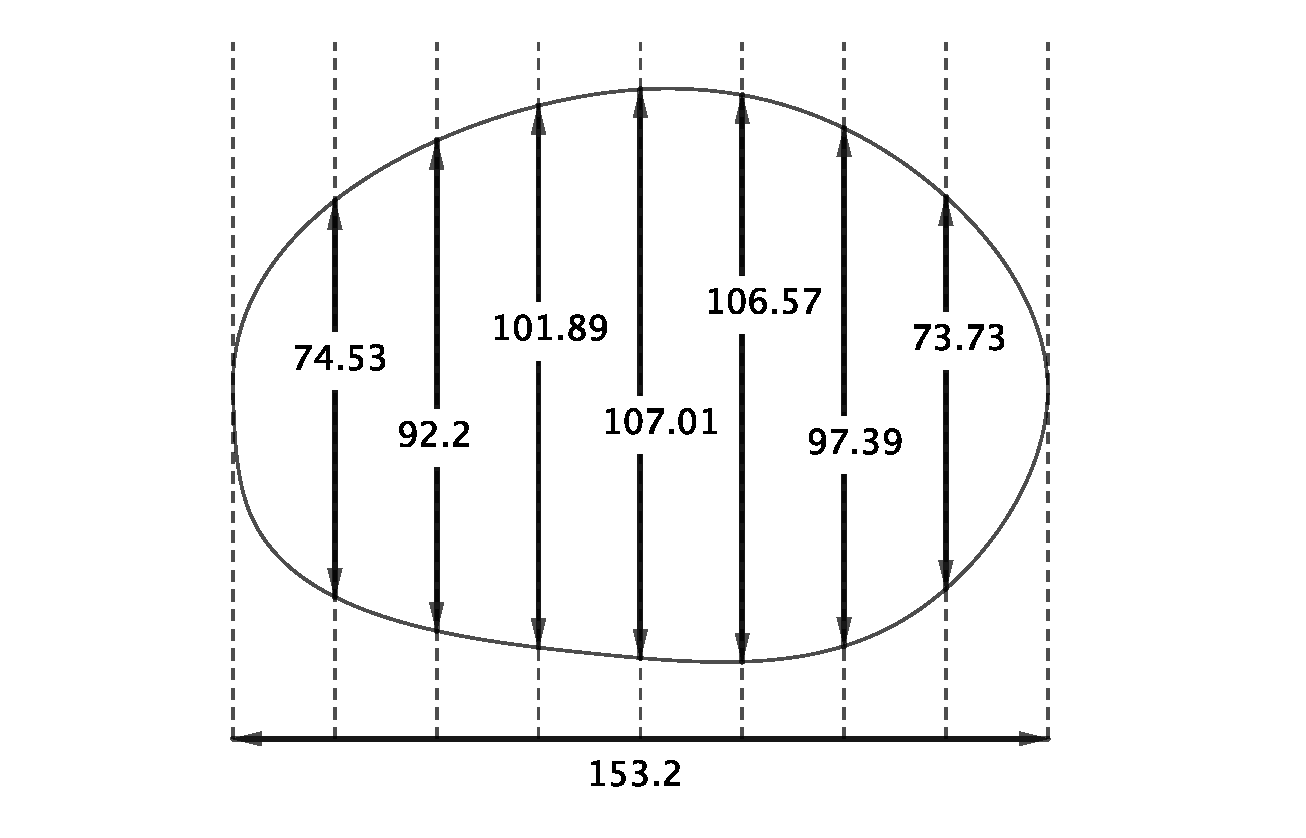
\includegraphics[height=8cm]{14/ike.pdf}
  \end{figure}

  池の幅 $153.2$ m を $8$ 等分して Simpson の公式を適用する.求める近似値は
  \[
    \begin{aligned}
      S_8 = \frac{153.2/8}{3} \Big(0.0 &+ 4\times 74.53 + 2 \times 92.2
      + 4\times 101.89 + 2\times 107.01 + 4\times 106.57 \\[1ex]
      &+ 2\times 97.30 + 4\times 73.73 + 0.0\Big) = 12894.84\cdots
    \end{aligned}
  \]
  となので,池の面積は約 $12895$ m$^2$ である.
\end{example}


\end{document}
